

\tikzset{every picture/.style={line width=0.75pt}} %set default line width to 0.75pt        

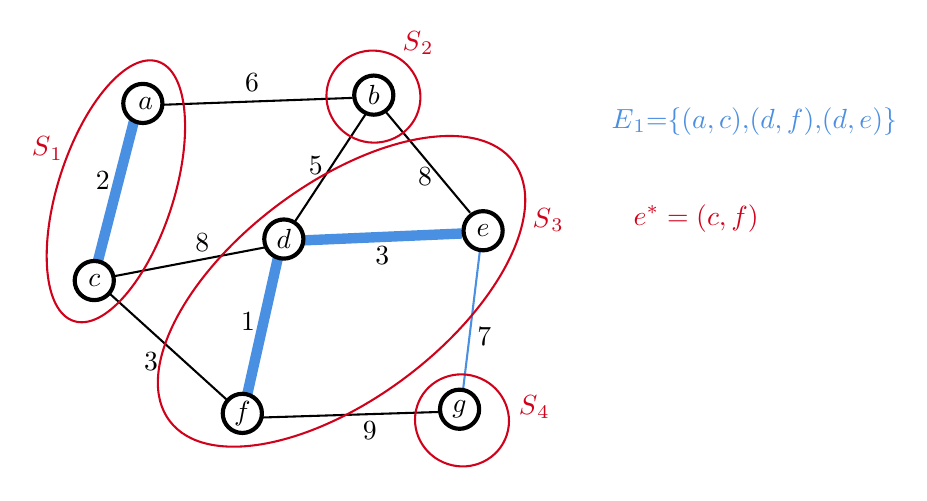
\begin{tikzpicture}[x=0.5pt,y=0.5pt,yscale=-1,xscale=1]
%uncomment if require: \path (0,371); %set diagram left start at 0, and has height of 371

%Straight Lines [id:da823970354045778] 
\draw [color={rgb, 255:red, 0; green, 0; blue, 0 }  ,draw opacity=1 ][line width=0.75]    (276,77) -- (337,150) ;
%Straight Lines [id:da271237396517352] 
\draw [color={rgb, 255:red, 0; green, 0; blue, 0 }  ,draw opacity=1 ][line width=0.75]    (186,298) -- (314,294) ;
%Straight Lines [id:da6657573604931601] 
\draw [color={rgb, 255:red, 0; green, 0; blue, 0 }  ,draw opacity=1 ][line width=0.75]    (76,208) -- (161,285) ;
%Straight Lines [id:da31661075744879486] 
\draw [color={rgb, 255:red, 0; green, 0; blue, 0 }  ,draw opacity=1 ][line width=0.75]    (79,196) -- (189,175) ;
%Straight Lines [id:da9969849240959807] 
\draw [color={rgb, 255:red, 74; green, 144; blue, 226 }  ,draw opacity=1 ][line width=3.75]    (94,84) -- (68,185) ;
%Straight Lines [id:da14506071047898028] 
\draw [color={rgb, 255:red, 0; green, 0; blue, 0 }  ,draw opacity=1 ][line width=0.75]    (114,72) -- (252,67) ;
%Straight Lines [id:da8946288202546534] 
\draw [color={rgb, 255:red, 0; green, 0; blue, 0 }  ,draw opacity=1 ][line width=0.75]    (262,78) -- (210,157) ;
%Straight Lines [id:da15496081521651384] 
\draw [color={rgb, 255:red, 74; green, 144; blue, 226 }  ,draw opacity=1 ][line width=3.75]    (198,183) -- (176,281) ;
%Straight Lines [id:da2163317830574415] 
\draw [color={rgb, 255:red, 74; green, 144; blue, 226 }  ,draw opacity=1 ][line width=0.75]    (344,178) -- (332,277) ;
%Straight Lines [id:da5391246746067021] 
\draw [color={rgb, 255:red, 74; green, 144; blue, 226 }  ,draw opacity=1 ][line width=3.75]    (331,165) -- (216,170) ;
%Shape: Ellipse [id:dp8079044569602617] 
\draw  [color={rgb, 255:red, 208; green, 2; blue, 27 }  ,draw opacity=1 ] (41.31,121.62) .. controls (58.12,69.84) and (89.51,33.63) .. (111.43,40.74) .. controls (133.35,47.86) and (137.49,95.6) .. (120.69,147.38) .. controls (103.88,199.16) and (72.49,235.37) .. (50.57,228.26) .. controls (28.65,221.14) and (24.51,173.4) .. (41.31,121.62) -- cycle ;
%Shape: Ellipse [id:dp9738354187366457] 
\draw  [color={rgb, 255:red, 208; green, 2; blue, 27 }  ,draw opacity=1 ] (197.42,144.88) .. controls (266.03,93.16) and (342.55,78.94) .. (368.33,113.13) .. controls (394.1,147.32) and (359.37,216.97) .. (290.75,268.7) .. controls (222.13,320.42) and (145.61,334.64) .. (119.84,300.45) .. controls (94.07,266.26) and (128.8,196.61) .. (197.42,144.88) -- cycle ;
%Shape: Ellipse [id:dp2276168529447603] 
\draw  [color={rgb, 255:red, 208; green, 2; blue, 27 }  ,draw opacity=1 ] (234.76,55.56) .. controls (240.41,38.13) and (259.49,28.7) .. (277.37,34.51) .. controls (295.25,40.31) and (305.16,59.14) .. (299.5,76.57) .. controls (293.85,94.01) and (274.77,103.43) .. (256.89,97.63) .. controls (239.01,91.83) and (229.1,72.99) .. (234.76,55.56) -- cycle ;
%Shape: Ellipse [id:dp3153590720909477] 
\draw  [color={rgb, 255:red, 208; green, 2; blue, 27 }  ,draw opacity=1 ] (298.76,289.56) .. controls (304.41,272.13) and (323.49,262.7) .. (341.37,268.51) .. controls (359.25,274.31) and (369.16,293.14) .. (363.5,310.57) .. controls (357.85,328.01) and (338.77,337.43) .. (320.89,331.63) .. controls (303.01,325.83) and (293.1,306.99) .. (298.76,289.56) -- cycle ;

% Text Node
\draw  [line width=1.5]   (346.38, 163) circle [x radius= 14.15, y radius= 14.15]   ;
\draw (346.38,163) node   [align=left] {$\displaystyle e$};
% Text Node
\draw  [line width=1.5]   (100.48, 71) circle [x radius= 14.15, y radius= 14.15]   ;
\draw (94.98,71) node [anchor=west] [inner sep=0.75pt]   [align=left] {$\displaystyle a$};
% Text Node
\draw  [line width=1.5]   (267.38, 65) circle [x radius= 14.15, y radius= 14.15]   ;
\draw (267.38,65) node   [align=left] {$\displaystyle b$};
% Text Node
\draw  [line width=1.5]   (65.38, 199) circle [x radius= 14.15, y radius= 14.15]   ;
\draw (65.38,199) node   [align=left] {$\displaystyle c$};
% Text Node
\draw  [line width=1.5]   (202.38, 169) circle [x radius= 14.15, y radius= 14.15]   ;
\draw (202.38,169) node   [align=left] {$\displaystyle d$};
% Text Node
\draw  [line width=1.5]   (172.38, 295) circle [x radius= 14.15, y radius= 14.15]   ;
\draw (172.38,295) node   [align=left] {$\displaystyle f$};
% Text Node
\draw  [line width=1.5]   (329.38, 292) circle [x radius= 14.15, y radius= 14.15]   ;
\draw (329.38,292) node   [align=left] {$\displaystyle g$};
% Text Node
\draw (64.24,118.06) node [anchor=north west][inner sep=0.75pt]   [align=left] {$\displaystyle 2$};
% Text Node
\draw (172.24,47.06) node [anchor=north west][inner sep=0.75pt]   [align=left] {$\displaystyle 6$};
% Text Node
\draw (266.24,172.06) node [anchor=north west][inner sep=0.75pt]   [align=left] {$\displaystyle 3$};
% Text Node
\draw (218.24,107.06) node [anchor=north west][inner sep=0.75pt]   [align=left] {$\displaystyle 5$};
% Text Node
\draw (136.24,163.06) node [anchor=north west][inner sep=0.75pt]   [align=left] {$\displaystyle 8$};
% Text Node
\draw (99.24,249.06) node [anchor=north west][inner sep=0.75pt]   [align=left] {$\displaystyle 3$};
% Text Node
\draw (169.24,220.06) node [anchor=north west][inner sep=0.75pt]   [align=left] {$\displaystyle 1$};
% Text Node
\draw (297.24,115.06) node [anchor=north west][inner sep=0.75pt]   [align=left] {$\displaystyle 8$};
% Text Node
\draw (257.24,299.06) node [anchor=north west][inner sep=0.75pt]   [align=left] {$\displaystyle 9$};
% Text Node
\draw (340,230.5) node [anchor=north west][inner sep=0.75pt]   [align=left] {$\displaystyle 7$};
% Text Node
\draw (437,72) node [anchor=north west][inner sep=0.75pt]   [align=left] {$\displaystyle \textcolor[rgb]{0.29,0.56,0.89}{E}\textcolor[rgb]{0.29,0.56,0.89}{_{1}}\textcolor[rgb]{0.29,0.56,0.89}{=}\textcolor[rgb]{0.29,0.56,0.89}{\{}\textcolor[rgb]{0.29,0.56,0.89}{(}\textcolor[rgb]{0.29,0.56,0.89}{a,c}\textcolor[rgb]{0.29,0.56,0.89}{)}\textcolor[rgb]{0.29,0.56,0.89}{,}\textcolor[rgb]{0.29,0.56,0.89}{(}\textcolor[rgb]{0.29,0.56,0.89}{d,f}\textcolor[rgb]{0.29,0.56,0.89}{)}\textcolor[rgb]{0.29,0.56,0.89}{,}\textcolor[rgb]{0.29,0.56,0.89}{(}\textcolor[rgb]{0.29,0.56,0.89}{d,e}\textcolor[rgb]{0.29,0.56,0.89}{)}\textcolor[rgb]{0.29,0.56,0.89}{\}}$};
% Text Node
\draw (18,93) node [anchor=north west][inner sep=0.75pt]   [align=left] {$\displaystyle \textcolor[rgb]{0.82,0.01,0.11}{S}\textcolor[rgb]{0.82,0.01,0.11}{_{1}}$};
% Text Node
\draw (286,17) node [anchor=north west][inner sep=0.75pt]   [align=left] {$\displaystyle \textcolor[rgb]{0.82,0.01,0.11}{S}\textcolor[rgb]{0.82,0.01,0.11}{_{2}}$};
% Text Node
\draw (380,145) node [anchor=north west][inner sep=0.75pt]   [align=left] {$\displaystyle \textcolor[rgb]{0.82,0.01,0.11}{S}\textcolor[rgb]{0.82,0.01,0.11}{_{3}}$};
% Text Node
\draw (370,280) node [anchor=north west][inner sep=0.75pt]   [align=left] {$\displaystyle \textcolor[rgb]{0.82,0.01,0.11}{S}\textcolor[rgb]{0.82,0.01,0.11}{_{4}}$};
% Text Node
\draw (453,142) node [anchor=north west][inner sep=0.75pt]   [align=left] {$\displaystyle \textcolor[rgb]{0.82,0.01,0.11}{e^{*} =( c,f)}$};


\end{tikzpicture}

